\chapter{Evaluation}
\label{c:discussion}
The research questions that are tackled in this thesis cover two primary objectives.
The first goal is to provide a visualization of program behavior at the abstraction level of objects that preservers the immediate character and low memory footprint of the underlying tracing framework.
The second goal is to provide a visualization that imparts this information in a perceivable manner and supports the developer in the understanding of the software system at hand.

Section \ref{s:DiscussionPerformance} gives an insight to which extent the first goal could be reached with the Squeak/Smalltalk implementation of our approach.
To validate that the extensions that had to be made to the tracing framework and the computational complexity introduced through the visualization do not jeopardize immediacy, an evaluation of the runtime performance is given in Section \ref{ss:DiscussionPerformance}.
An evaluation of the additional memory consumption that our specialized variant of  step-wise run-time analysis brings along is presented in Section \ref{ss:DiscussionSpace}. 
The achievement of the second goal is examined with the help of a user study which is presented in Section \ref{s:DiscussionEvaluation}.

In addition, the limitations of our approach and its applicability to other programming languages and environments are discussed in Section \ref{s:DiscussionLimitations}.

\section{Performance Evaluation}
\label{s:DiscussionPerformance}
Research results already have shown that the step-wise run-time analysis approach that serves as a basis of \textsc{PathObjects} enables the immediate exploration of a programs runtime while maintaining a low memory footprint \cite{perscheid_immediacy_2010}.
To ensure that the computational extra work required for visualizing recorded object interactions preserves the immediate character of this approach, we evaluated the runtime performance of our implementation.
The results show that more than 75\% of the examined unit tests can be presented to developers in less than two seconds, and more than 95\% take no more than ten seconds.
Since \textsc{PathObjects} also introduces additional tracing effort, we also analyzed its memory requirements.
This evaluation shows that the additional memory consumption is lower than 1MB even in worst-case scenarios.

\subsection{Evaluated Projects}
\label{ss:DiscussionProjects}
In order to get a meaningful performance estimation, four real-world software projects with different backgrounds were chosen as a basis for the measurements.
The extent of those projects (cf. Table \ref{t:EvaluationProjects}) ranges from roughly 210 methods in 16 classes to almost 1900 methods in over 210 classes.
\textsc{Seaside}\footnote{\url{http://seaside.st}, last checked \today} is a full-fledged, industry grade web application framework.
\textsc{DicThesauruasRex}\footnote{\url{https://www.hpi.uni-potsdam.de/hirschfeld/trac/SqueakCommunityProjects/wiki/dicThesaurusRex}, last checked \today} is the result of an undergraduate student project which adds spelling correction and synonym search facilities to the Squeak development environment.
\textsc{SUnit}\footnote{\url{http://sunit.sourceforge.net/}, last checked \today} is the de-facto standard for unit testing frameworks in Smalltalk environments and constitutes a landmark of test-driven development.
The \textsc{System Browser}\footnote{\url{http://wiki.squeak.org/squeak/673}, last checked \today} is the fundamental development tool in Squeak images that allows to browse and edit the source codes of the image.

\begin{table}
\centering
\begin{tabular}{lcccccc}
\toprule[1.5pt]
\phantom{abc} & \phantom{abc} & \multicolumn{2}{c}{Classes} & \phantom{abc} & \multicolumn{2}{c}{Methods}  \\
\cmidrule{3-4} \cmidrule{6-7}
Project    && System & Test && System & Test \\
\midrule
\textsc{Seaside-Core}		&&	163	&	49	&&	1409	&	458	\\
\textsc{DicThesaurusRex}	&&	23	&	14	&&	204		&	69	\\
\textsc{SUnit}				&&	8	&	8	&&	160		&	49	\\
\textsc{System Browser}		&&	54	&	13	&&	1204	&	162	\\
\bottomrule[1.5pt]
\end{tabular}
\caption[Evaluated Software Systems]{Scale of the software systems that served as a basis for the performance evaluation.}
\label{t:EvaluationProjects}
\end{table}

\subsection{Runtime Performance}
\label{ss:DiscussionPerformance}
Most traditional dynamic analysis tools refrain from information presentations that require complex computations.
Instead, they rely on sequence diagrams or similar visualizations that can be generated trivially.
In contrast, the major bottleneck of our approach can be accounted to the hierarchical graph drawing that is performed in order to render object interactions.

The algorithm implemented by \textsc{Graphviz} has been designed with its interactive application in mind and generally performs fast enough therefor \cite{gansner_technique_1993}.
Nevertheless, its runtime is heavily dependent on the specific structure of the graph at hand.
Precisely, the edge crossing minimization problem is NP-hard and the applied heuristic requires quadratic time in the number of nodes in the worst case \cite{tamassia_handbook_2013}.
This case eventuates when edges span the maximum possible number of ranks.
An example graph with $n$ ranks that shows this characteristic is depicted in Figure \ref{fig:graph-worst-case}.

Since it is practically impossible to predict to which degree call trees of test cases conform to this structure, the four real-world projects depicted in Section \ref{ss:DiscussionProjects} have been used to carry out an evaluation of the runtime behavior of our approach.

\begin{figure}[b]
	\centering	
	\digraph
	[scale=0.8]{worstCaseRuntimeComplexity}
	{
		margin=0
		nodesep=0.4
		node [style=rounded, shape=box, fontsize=11, height=0.4]
		n1 [label=<N<SUB>1</SUB>>]
		n2 [label=<N<SUB>2</SUB>>]
		nx [label="...", style="rounded,dotted"]
		nn1 [label=<N<SUB>n-1</SUB>>]
		nn [label=<N<SUB>n</SUB>>]
		n1->n2
		n2 -> nx [style=dotted,arrowhead=onormal]
		nx->nn1 [style=dotted,arrowhead=onormal]
		nx -> nn [style=dotted, arrowhead=onormal]
		nn1-> nn
		n1 -> nn
		n2 -> nn
		{rank=same n1 n2 nx nn1 nn}
	}
	\caption[Example Graph that Entails Worst Case Runtime Complexity]{Example graph that entails the worst case runtime complexity of $\mathcal O(n^2)$.}
	\label{fig:graph-worst-case}
\end{figure}

\subsubsection{Evaluation Procedure}
For each test case of the evaluated software systems, a time measurement was taken.
The selection of a test case constitutes the start of a measurement, and the completion of the start-up of \textsc{PathObjects} its end.
In other words, the measurements include all operations that have to be performed before the developer can start analyzing a test case through \textsc{PathObjects}.
Namely these are the execution of a shallow analysis, the initialization of all user interface elements, the computation of a graph layout, and its application to the generated diagram.
Between each measurement, garbage collection was triggered multiple times in order to prevent unintended side effects through growing memory consumption.

All measurements were performed on an Intel\copyright{} Core\texttrademark{}  i7-2620M CPU @ 2.70GHz.
The Squeak image version 4.4-12327 was executed on a Windows 7 x64 host operating system with the Croquet Closure Stack VM, version StackInterpreter VMMaker-oscog-EstebanLorenzano.237\footnote{\url{http://source.squeak.org/VMMaker/VMMaker-oscog-EstebanLorenzano.237.mcz}, last checked \today}. 
This combination of CPU and VM performs at 528.1 million bytecodes/sec and 27.3 million sends/sec in the Squeak Tiny Benchmarks. \textsc{Graphviz} served as graph drawing engine and was present in version 2.34.

\subsubsection{Results}

\begin{figure}[tb!]
	\centering
	\includegraphics[width=0.9\textwidth]{../plots/05-Runtimes}
	\caption[Runtime Performance of \textsc{PathObjects}]{Runtime performance of \textsc{PathObjects} with various projects (whiskers indicate 2.5th and 97.5th percentiles).}
	\label{f:DiscussionRuntime}
\end{figure}

The results of the measurement are depicted in Figure \ref{f:DiscussionRuntime}.
The start-up time is faster than one second in more than 50\% of all measured test cases.
More than 75\% of all measurements are below two seconds.
In the case of \textsc{DicThesaurusRex} and \textsc{SUnit}, even the third quartiles are below one second.
The outliers reach up to 34 seconds with the worst-case occurring in the \textsc{Seaside-Core} project.

In comparison to the majority of test cases, the start-up times of the outliers are significantly slower.
However, when compared to traditional dynamic analysis tools (cf. Section \ref{ss:BackgroundAnalysisProblems}), the results nevertheless are available considerably faster.
Furthermore, those test case are rather comprehensive in terms of the number of objects and messages, and it is doubtful that developers want to visualize these amounts of data in their entirety.
Consequently, a possible solution to speed up the visualization of these test cases would be to provide an alternative entry point that allows developers to specify entities of interest through the \textsc{PathView} filter.
Thus, the graph that has to be processed during the graph drawing phase could be narrowed down before the first layout computation.

In summary, it can be said that the total time required for tracing and processing is entirely satisfactory in case of the four investigated projects.
These projects are real-world software systems rather than synthetic benchmarks.
Hence, it can be concluded that even though our approach entails operations with high computational complexity, it still is suitable to achieve considerably better performance compared to traditional dynamic analysis tools.

\subsubsection{Threats to Validity}
The runtime measurements have been performed with the help of the \inlinecode{timeToRunWithoutGC} method provided by \inlinecode{BlockClosure}, which has two implications.
First, the precision of the measurement is limited by the precision of the millisecond clock of the Squeak image.
Another side effect of measuring clock time instead of CPU time is that other running operating system processes can have an effect on the results.
But as millisecond precision is not important for our evaluation, both limitations are acceptable.

The second implication is that in practice, the start-up time of \textsc{PathObjects} will be slightly worse than depicted by the results of the runtime evaluation.
However, garbage collection should not be of major importance during the start-up phase.
Objects are not created and destroyed excessively through the tracing framework, so the main parts that are qualified for garbage collection are the ones of the system under investigation.
Furthermore, the start-ups are short running tasks.
Even if garbage collection would account for a significant share of the runtime, the overall start-up time would still be fast enough in the majority of cases.

Apart from that, a total of eight test cases originating from all four systems had to be excluded from the measurement, since they showed non-deterministic or non-terminating behavior.
However, these exceptions only amount to 1.0\% of the total number of test cases and thus can hardly invalidate the overall result of the runtime evaluation.

\subsection{Space Consumption}
\label{ss:DiscussionSpace}
As pointed out in Section \ref{s:BackgroundAnalysis}, one major problem of dynamic analysis techniques is the huge amount of data arising during tracing runs.
For that reason, the step-wise run-time analysis approach has been proposed as tracing technique with considerably lowered space requirements \cite{perscheid_immediacy_2010}. 
This approach also serves as a basis of \textsc{PathObjects}, but additional tracing effort had to be introduced to allow for the reconstruction of object interaction diagrams from those traces.
Therefore, an estimation of the additional space consumption \textsc{PathObjects} adds on top of the underlying tracing framework is presented in this section.

\subsubsection{Evaluation Procedure}
The main memory consumption of a specific part of the system is hard to measure exactly in a garbage collected environment like the Squeak virtual machine.
For that reason, the space requirements are estimated by means of theoretical deduction.
Figure \ref{fig:DiscussionStructure} depicts the basic components \textsc{PathObjects} traces consists of in the form of a simplified class diagram.

Each occurring object is represented by a proxy object that basically consists of an integer identifier and a pointer to its type.
Sent messages are represented by instances of the \inlinecode{Message} class.
They consist of pointers to the preceding and succeeding messages as well as a collection of integer object identifiers.
This collection includes identifiers for the sender and receiver of a message, its arguments, and for its return value.
In case of the \inlinecode{ObjectProxy} and \inlinecode{Message} classes, there is an overhead of two words for each object instance consumed by the object header.
Since all attributes are either integer values or pointers to other objects, the size of each attribute can be assumed to be one word.
The size of the \inlinecode{involvedObjects} collection has a constant part of four words for object headers and attributes and three words for the identifiers for sender, receiver, and return value, but ultimately depends on the number of arguments of the according message.
In other words, the space consumption of our traces is dependent on the number of objects, the number of messages, and the number of arguments of each message.

Taken as a whole, the space consumption (in words) can be expressed as a function $s(o,m)$ of the number of objects $o$ and the number of messages $m$:
\begin{equation}
s(o,m)=o*4 + m*5 + \sum_{n=1}^{m} (7 + a(M_n))\label{eq:SpaceConsumptionWords}
\end{equation}
Thereby, the number of arguments of a message $M_n$ are represented by the function $a$.
Since a word consumes four bytes in the virtual machine we used, the total space consumption in kilobytes $s_{kB}$ can be calculated with the help of formula \ref{eq:SpaceConsumptionBytes}. 
\begin{equation}
s_{kB}(o,m) = \frac{4 * s(o,m)}{1000}\label{eq:SpaceConsumptionBytes}
\end{equation}
To get a reasonable estimation of the three variable parts $o$, $m$, and $a(M_n)$, their actual numbers in the case of the four evaluation projects have were determined.

\usetikzlibrary{positioning,shapes,shadows,arrows}
\tikzstyle{class}=[
	rectangle,
	draw=black,
	text centered,
	anchor=north,
	text=black,
	text width=3cm,
	minimum height=0.6cm,
	shading=axis,bottom color=black!20,top color=white,shading angle=45
	]
	
\tikzset{every node/.style={draw}}

\begin{figure}[tb!]
	\centering
	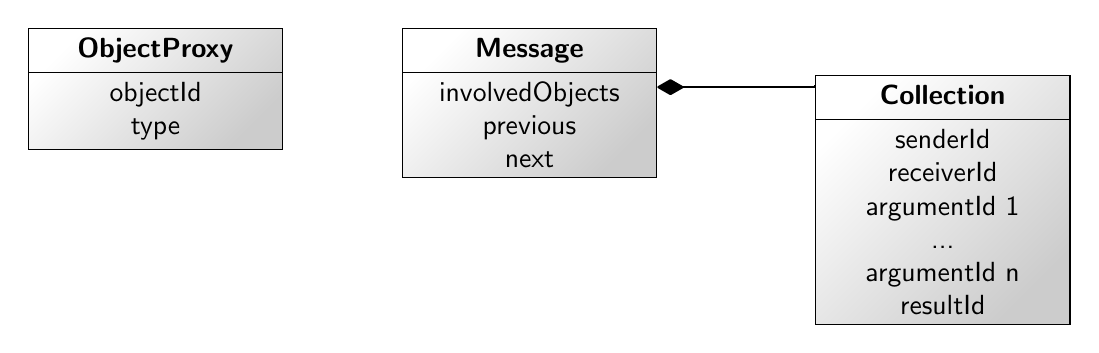
\begin{tikzpicture}[node distance=2cm, font=\sffamily]

		\node (ObjectProxy) [class, rectangle split, rectangle split parts=2] {
				\textbf{ObjectProxy}
				\nodepart{second} objectId \\ type
		};

		\node (Message) [class, rectangle split, rectangle split parts=2, below right=0cm and 1.5cm of ObjectProxy.north east] {
			\textbf{Message}
			\nodepart{second} involvedObjects \\ previous \\ next
		};
		
		\node (Collection) [class, rectangle split, rectangle split parts=2, below right=0.6cm and 2cm of Message.north east] {
			\textbf{Collection\vphantom{g}}
			\nodepart{second} senderId \\ receiverId \\ argumentId 1 \\ ... \\
			 argumentId n \\ resultId
		};
		
		\draw[>-, >=diamond, shorten >=1pt, thick] 
    		(Message.east) ++(0,0.2) -| ([yshift=1.5cm]Collection.west); 
			
	\end{tikzpicture}
	\caption[Memory Consuming Components of \textsc{PathObjects} Traces]{Memory consuming components of \textsc{PathObjects} traces.}
	\label{fig:DiscussionStructure}
\end{figure}

\subsubsection{Results}
The results of the evaluation are depicted in Figure \ref{fig:DiscussionSpace}.
It shows the space consumption that is introduced through \textsc{PathObjects} in addition to the data that is collected through the underlying tracing framework.
All results were calculated by applying formula \ref{eq:SpaceConsumptionBytes} to the specific values of $o$, $m$, and $a(M_n)$ which were determined per test case.

In each of the evaluated projects, over 50\% of the test cases imply less than 10kB of additionally collected data.
More than 97.5\% of all evaluated test cases require less than 200kB in addition.
The worst case occurs in a unit test of the Squeak System Browser.
In this case, the additional space requirements add up to around 900kB.

A performance analysis of step-wise run-time analysis already has shown that it maintains a low memory footprint during tracing \cite{perscheid_immediacy_2010}.
With the worst case introducing less than 1MB of additional tracing data, it can be concluded that the space consumption overhead that is required for the reconstruction of object interactions is negligible.

\begin{figure}[tb!]
	\centering
	\includegraphics[width=0.9\textwidth]{../plots/05-SpaceConsumption}
	\caption[Space Requirements Introduced Through \textsc{PathObjects}]{Additional space consumption introduced through the tracing requirements of \textsc{PathObjects} (whiskers indicate 2.5th and 97.5th percentiles).}
	\label{fig:DiscussionSpace}
\end{figure}

\subsubsection{Threats to Validity}
The calculated memory consumption should be interpreted as lower limit of the values that are reached in practice.
Although the overhead implicated by object instances themself in the Squeak virtual machine is taken into consideration, the memory consumption will effectively be higher than determined by our calculations.
First, the memory overhead the virtual machine itself introduces to manage objects can not be considered with the chosen approach.
Second, memory allocation is rather performed in blocks than with byte precision.
Consequently, the actual memory consumption depends on the number of blocks that have to be allocated to satisfy the requirements.
Third, a similar problem is memory alignment or rather data misalignment, which can cause objects to consume more memory than necessary.
These pitfalls of memory management can not be taken into consideration reasonably with our theoretical deduction.

Nonetheless, all those factors will not add up to invalidate the basic results of the evaluation.
Even when assuming huge deviations that lead to a tenfold memory consumption compared to the result of formula \ref{eq:SpaceConsumptionWords}, the consumption still would lie within a range of a few megabytes.
Nowadays, this is a scale that can be demanded from hardware with clear conscience.

\clearpage
\section{User Study}
\label{s:DiscussionEvaluation}
In order to validate that \textsc{PathObjects} can help developers to build a understanding of software systems and their behavior better than with the help of traditional tools alone, a user study has been conducted.
For that purpose, five tasks concerning the \textsc{DicThesaurusRex} project were derived from questions that reportedly arise often during software development.
Study participants were challenged to solve these tasks, whereby the target software system was previously unknown to them.
The results of the study show that participants which were allowed to use \textsc{PathObjects} showed a higher degree of comprehension for each task in comparison to those who used the Squeak standard tools or \textsc{PathFinder}.

\subsection{Participant Profile}
Twelve undergraduate and graduate students with a professional background in object-oriented programming in general and Squeak/Smalltalk in particular were invited to take part in the user study.
All participants had between four and ten years of experience with object-oriented programming languages and two to six years of experience with Squeak/Smalltalk.
Furthermore, all participants reached good or very good grades in a mandatory software engineering lecture, which included a Smalltalk programming project as major component of the overall grade (six participants were graded A, four participants were graded A-, and two participants were graded B+).
None of the participants had any considerable prior experience with \textsc{PathFinder} or \textsc{PathObjects}.

The twelve participants were randomly divided into three groups, whereby each group was allowed to use a different set of tools to solve the appointed tasks.
The participants in group A were asked to use only the standard tools of the Squeak environment, including, but not limited to the source browser, test runner, debugger, and workspace.
The participants in group B were prompted to use \textsc{PathFinder}, the back-in-time debugger that implements step-wise run-time analysis (cf. Section \ref{ss:BackgroundTracing}).
Similarly, the participants in group C were challenged to solve the tasks with the help of our implementation of \textsc{PathObjects}.
Theoretically, the probands in groups B and C were also allowed to use the Squeak standard tools.
However, the only tool that was used sporadically in addition to the primary tool of the respective group was the source browser.

\subsection{Evaluated Tasks}
The questions developers ask during software development activities are a research area of its own.
Among others, Sillito et al. and LaToza et al. have published results from user studies on this topic \cite{sillito_asking_2008, latoza_hard--answer_2010}.
From the questions that were determined by these studies, five were selected and adapted to comprehension tasks regarding \textsc{DicThesaurusRex}.
This project provides spell checking and thesaurus functionalities for various standard tools of the Squeak environment.
It is the result of an undergraduate student project and features a sufficient unit test suite.

However, the range of subjects in these user studies is not limited to object-oriented programming.
For instance, generic questions such as which design would be the best choice to implement a functionality also are part of the outcome of these studies.
Consequently, we only used those questions as a basis which appeared to be answerable with our implementation of \textsc{PathObjects}.

\paragraph{Task 1} The project contains a parser class that is used to extract single words from designators which are named in camel case style, namely \inlinecode{DTRCamelCaseParser}.
Participants were asked to describe how this parser works, and could score a maximum of eight points that cover the cornerstones of this algorithm.
The test case \inlinecode{testWholeWordParsing} that spans a suitable scenario was provided as entry point.
The difficulties of this task are the high number of execution branches that have to be followed, and the handling of edge cases like acronyms or special characters.

\paragraph{Task 2} The thesaurus implementation creates instances of \inlinecode{DTRThesaurusEntry} that map words to their synonyms.
They have an instance variable named \inlinecode{pos} which is used to mark the word class.
Participants were asked to determine the purpose of this variable.
However, since this variable is neither documented nor actually used at all, their is no straightforward solution strategy.
The answer had to be selected from a given list of possible values, with \inlinecode{noun} being the only correct entry.
Consequently, participants could score one point on this task.

\paragraph{Task 3} The search for synonyms exhibits differing time complexities depending on whether the search term is present in the thesaurus or not.
Since the implementation is based on a \inlinecode{Dictionary}, a failing lookup of a search term is performed in constant time.
In contrast, the lookup of actual synonyms is dependent on the number of found thesaurus entries due to the post-processing that is performed for each match.
Participants were asked to give duration estimations for searches that do and do not return results, whereby they also were allowed to make use of profiling utilities.
The answers had to be selected from a given list of time values, and consequently the maximum possible score for this task was one point per case, or respectively two points in total.
Two test cases were provided as entry points, namely \inlinecode{testSynonymsOf} and \inlinecode{testEmptySynonymsOf}.

\paragraph{Task 4} The spell checking module provides a method to test strings for spelling errors, namely \inlinecode{checkSpellingOf:}.
This method uses the camel case parser to split the input string into single words.
Participants were asked to find out how many parser instances are used to check the spelling of a given input string, and to state reasons for their answer.
The problem with this scenario is that the source code strongly suggests that only one parser instance is used.
However, the implementation creates one to three further instances for each found word, depending on whether spelling errors are found or not.
Participants could score a maximum of five points: one for the correct number of instances, two for the locations where they get created, and two for the reasons that lead to the creation of those additional instances.
The unit test \inlinecode{testCheckSpellingOf} was provided as entry point.

\paragraph{Task 5} In this task, the participants were challenged to find the most recent changes of the spell checking process, which already served as object of investigation in Task 4.
For instance, such information can be relevant when features break after merging new commits.
To solve the task, the three methods with the most recent alteration dates had to be named.
Consequently, the maximum possible score for this tasks was three points.
There are two different problems with this task.
First, participants have to identify the methods that are involved in the spell checking process, or in other words, those that are called transitively starting from the \inlinecode{checkSpellingOf:} method.
Second, the identified methods have to be compared with regards to their alteration dates.
Again, the \inlinecode{testCheckSpellingOf} was provided as entry point.

\subsection{Experimental Setup}
Participant were challenged separately in dedicated sessions.
Thereby, the workplace, hardware, and Squeak image\footnote{This image provided Squeak 4.4, \textsc{PathObjects} 0.2 (available online at \url{https://github.com/leoschweizer/PathObjects/releases/tag/v0.2-Milestone}, last checked \today), and \textsc{PathTools} 1.7} were identical for each participant.
Consequently, it can be ruled out that factors like screen real estate or processing speed had an influence on the performance of the participants. 
During the whole time of an experiment session, the study investigator was present.
Foregoing the actual user study, all participants were asked to solve an introductory task, which involved the implementation of a single linked list and some simple operations.
The task was finished as soon as all provided unit tests were satisfied.
The purpose of this task was to harmonize the proficiency of the participants in dealing with the provided Squeak environment, and to revive their knowledge about Squeak/Smalltalk.

In the case of groups B an C, each experiment then started with a 15-minute introduction of the respective tools, since none of the participants had any prior experience with them.
All features that could help to solve the tasks were explained, and participants were prompted to familiarize themselves with these features. 
This step could be skipped in the case of group A, since all participants were sufficiently familiar with the Squeak environment.
Afterwards, a brief introduction into the \textsc{DicThesaurusRex} project was given.
The spell checking and synonym search functionalities were demonstrated, but no parts of the source code or other implementation details were revealed.

Subsequently, the tasks were handed to participants on by one in written form.
All task descriptions were kept undisclosed, with the exception of the current one.
In other words, participants were only allowed to read the next task after finishing the previous one.
The tasks were handed out in the exact same order in each experiment.
Participants were allowed to spend as much time as desired on each task, and a task was regarded as finished as soon as participants were confident in terms of the comprehensiveness of their answer.

For each task, two measures were utilized to grade the performance of participants, namely the processing time and the degree of comprehension.
The measurement of the processing time started with the handover of a task, and ended when participants declared their answer as finished.
The degree of comprehension was measured with the aid of a score-based grading of the answers participants gave, and expresses the percentage of points that were scored on a task (cf. Definition \ref{eq:UserEvaluationDc}).

\begin{equation}
Comprehension(user, task) = \frac{Score(user, task)}{MaximumScore(task)}\label{eq:UserEvaluationDc}
\end{equation}

\subsection{Results and Interpretation}

\begin{figure}[tb!]
	\centering

	\includegraphics[width=1.0\textwidth]{../plots/05-UserEvaluation}
	\caption[Results of the User Study]{Performance of the participant groups (A: Squeak standard tools, B: \textsc{PathFinder}, C: \textsc{PathObjects}) per task, measured by degree of comprehension (higher is better) and processing time (lower is better); whiskers indicate the lowest and highest occurrences.}
	\label{fig:DiscussionStudyResults}
	
\end{figure}

The results of the user study are depicted in Figure \ref{fig:DiscussionStudyResults}.
For each task, the required processing time is broken down by the three participant groups, and related to the determined degree of comprehension.

\paragraph{Task 1} Strikingly, the mean time participants in group B spent on this task is almost six minutes higher than that of group A.
The reason for this phenomenon is that participants in group A had to follow a lot of branches and transitive calls manually, and simply discontinued to do so when the further investigation seemed to cumbersome.
In contrast, \textsc{PathFinder} displays the whole scenario at once, and participants had an intuitive understanding whether they gathered all relevant details.
Surprisingly, this did not lead to a noticeable increase in the degree of comprehension.
The participants in group C also were slower in comparison to group A.
But in return, the mean degree of comprehension of this group is 0,31 points higher.
This can be explained by the fact that many implementation details of the algorithm under investigation can be revealed by simply expanding the object state indicator of the covered camel case parser instance, and by stepping through the execution trace.
This approach is not supported by \textsc{PathFinder}, and impossible with the standard development tools alone.

\paragraph{Task 2} All groups reached the maximum degree of comprehension of 1.0 on this task.
However, the participants in group C were noticeably faster than the other two groups. 
One reason for this phenomenon is that while the developers in group A had to browse senders manually for a meaningful occurrence, the participants in group C simply used the search function of \textsc{PathObjects}, and explored the argument of a call of the \inlinecode{pos:} method.
Even though \textsc{PathFinder} also provides a search functionality, the participants of the respective group instead expanded the complete call tree and looked for occurrences of this setter method manually.

\paragraph{Task 3} The first thing to be noticed is that groups B and C managed to reach the maximum degree of comprehension, while two participants in group A failed to do so.
The reason for this shortage lies in the different solution strategies that were applied by participants in group A.
One participant used the profiling functionality of the test runner, which itself uses the \inlinecode{MessageTally} profiler.
The other participant used this profiler directly.
However, \inlinecode{MessageTally} is a sampling profiler, and the measurement of the execution of an unsuccessful search for synonyms is too fast to be captured by a sample.
Consequently, both participants guessed a value based on their measurement of a successful search, but were at fault in doing so.
The other participants in group A did time measurements with the help of \inlinecode{millisecondsToRun:} manually, and got correct results in this way.
What also attracts attention is that participants in group B were faster then those in group C.
This can be accounted to the fact that \textsc{PathFinder} includes a full-fledged profiling functionality that displays the actual measurement values to developers.
In contrast, the information layers of \textsc{PathObjects} do not display absolute values in the current implementation, and participants had to look up colors in a color scale manually in order to get an estimation.

\paragraph{Task 4} As depicted in the task description, the source code alone misleadingly suggests that only one instance of the camel case parser is used.
And as a matter of fact, all participants in group A only found this single instance.
In contrast, only one participant in group C failed to name all instances, but at least understood that the number of instances is dependent on the number of input words and spelling errors.
Although \textsc{PathFinder} also offers a view that distinguishes object identities, two participants nevertheless failed to identify more than the obvious occurrence.
They did not expand the call tree far enough to stumble across the other instances, and were under the impression that only one instance was used throughout the call tree.
As opposed to this, \textsc{PathObjects} presents a map of objects, and participants had an immediate overview of this scenario.
The reason that participants in group A were noticeably faster than the other two groups is that they did not spend any time to comprehend the reasons for the creation of the other instances, since they were not even aware of their existence.
In other words, the participants in group C spent more time on this task, but did not draw wrong conclusions about the behavior of the system.

\paragraph{Task 5} As it was expected, the participants in group A needed significantly more time to solve this task in comparison to the other two groups.
The reason is that they had to follow the transitive method calls of the spell checking process manually to find all involved methods, while \textsc{PathFinder} and \textsc{PathObjects} provide an overview of those methods.
The participants in group C in turn were noticeably faster than group B since the participants of the latter group had to look up all alteration dates manually.
In contrast, different solution strategies involving information layers were used by the participants of group C which directly showed the most recently changed methods.
What also strikes the eye is that participants in group A were rather unsuccessful in their search, while groups B and C show a comparable degree of comprehension.
However, the participants in group C required only around half of the mean time in comparison to group B.

\paragraph{Summary}
In comparison to the participants of group A, those that were allowed to use our implementation of \textsc{PathObjects} show a higher degree of comprehension of each evaluated task.
The sole exception is Task 2, were all participants of the three groups reach the maximum score.
Furthermore, the participants in group C required less time to gain this degree of comprehension in three out of five tasks.
The mean processing time of group A is lower in the case of Task 1 and Task 4, but this advantage comes at the cost of a distinctly reduced degree of comprehension.
The participants that were allowed to use \textsc{PathFinder} outperform group C only in the case of Task 3.
This result can be explained by the fact that \textsc{PathFinder} includes a full-fledged profiling functionality, which does not apply to \textsc{PathObjects}.
Furthermore, profiling is an activity that is not bound to the concepts of object-orientation.
In summary, it can be said that \textsc{PathObjects} successfully assisted participants in the evaluated tasks.

\subsection{Threats to Validity}
\paragraph{Internal Validity}
Generally speaking, the scale of the chosen subject project and the Smalltalk context could limit the overall applicability of our findings.
However, \textsc{DicThesaurusRex} is a real-world software project, and has not been developed for the purpose of our user study.
And although this fact alone is not sufficient to guarantee the usefulness of our concept with arbitrarily scaled software systems and different programming languages, the results still indicate worthwhile directions for further research on its general applicability.
Apart from that, our experimental setup can not guarantee the elimination of selection and experimenter bias.
Even though participants were selected on the basis of their relevant experiences and assigned to the different groups randomly, we cannot foreclose that differences in their mental abilities had an impact on the mean performance of the compared groups.
To rule out this factor, the user study would have to be conducted with a larger number of participants.
Since the user study was supervised by the implementer of \textsc{PathObjects} and was not conducted in a double blinded manner, it also cannot be foreclosed that experimenter bias had an influence on the performance characteristics of participants.

\paragraph{External Validity}
Although we tried to equalize the situational specifics for all participants, it still cannot be ruled out that they limit the generalizability of our findings.
All participants dealt with the tasks at the same workplace with the same technical equipment.
However, factors like ambient sounds, fitness depending on the time of the day, the general wellbeing of participants, and others were beyond our control.
Furthermore, not all participants were accustomed to the specifics attributable to the Windows operating system, such as the keyboard layout or shortcuts.
And although the introductory task was meant to harmonize the proficiency in dealing with the target system, some participants still might have benefited from previous knowledge.

\clearpage
\section{Discussion}
\label{s:DiscussionLimitations}
The operation of our implementation and the underlying tracing mechanism take some preconditions for granted whose non-compliance could potentially render them non-functional.
First, some restrictions apply when dealing with systems that use the metaprogramming and reflection capabilities of the Squeak environment.
However, they can be accounted to the implementation of the tracing framework, and do not invalidate the \textsc{PathObjects} concept itself.
Second, test coverage is an important factor for the usefulness of our current implementation, since only test cases are supported as entry points. 
Third, our concept relies on some test quality criteria, namely fast execution times and strict determinism.
Tests that do not comply to these properties are not suited for the use with \textsc{PathObjects}.

Apart from that, the fact that our implementation targets a niche environment raises the question to which extent the concept is applicable to other programming languages and environments.
However, there are no assumptions or preconditions in our concept that are specific to  Squeak/Smalltalk and thus would limit the applicability to this environment.

\subsection{Metaprogramming and Reflection}
\label{ss:DiscussionLimitationsMeta}
The utilization of metaprogramming and reflection capabilities within the system under observation does not necessarily pose a problem, neither on the conceptual nor on the technical level.
However, the underlying tracing approach based on method wrappers is not very resistant to structural changes that can be caused by the usage of those capabilities.

For instance, our implementation collects values of the program counter during tracing in order to permit the highlighting of the current message send within the corresponding method.
For that purpose, it browses the call stack, and expects a specific structure while doing so.
All method calls that originate from the tracing framework have to be skipped in order to find the actual call context and thus the appropriate program counter value.
If a program under observation manipulates the call stack, for instance by using method wrappers itself, the assumptions made about the sequence of tracing framework calls no longer hold true.
Consequently, information that is collected during such tracing runs would be incorrect.

Other tracing approaches might be less susceptible to such interferences, especially if traces are built via external observation of the target system, as is the case with the utilization of debug interfaces or with tracing on the virtual machine level.
However, the application of that sort of reflective capabilities is rarely found in practice.
Therefore, the limitations that are introduced in conjunction with tracing on the basis of method wrappers are acceptable.
Furthermore, these limitations do not invalidate the concept of \textsc{PathObjects} itself, since it might just as well be implemented with other, more resistant tracing approaches.

\subsection{Reliance on Test Coverage}
\label{ss:DiscussionLimitationsCoverage}
Since only test cases can serve as reproducible entry points in our current prototypic implementation, only those parts of a system can be visualized that are covered by at least one test case.
In practice, this means that not all entities and execution branches that are actually in use during productive executions of the system can necessarily be visualized with existing tests.
Nonetheless, it is also feasible to write specific unit tests for the soul purpose of visualization.
Such a test then can be seen as the description of a scenario that the user wishes to examine through our tool.
Admittedly, this strategy requires the user to already have a certain degree of knowledge, which might not apply when dealing with previously unknown systems.
In such cases, one might not be able to construct a working scenario.

However, the concept of \textsc{PathObjects} is not limited to test cases.
The underlying tracing approach works with any reproducible entry point into program behavior.
Consequently, the restriction to test cases is a limitation of the implementation rather than of the concept itself.

\subsection{Reliance on Test Quality}
\label{ss:DiscussionLimitationsTestQuality}
The best practices for unit testing and the characteristics unit tests should display enjoy broad consent throughout the agile software development community.
To name a few, they are supposed to be isolated, to be free of side-effects, to run fast, and to be reproducible, automated and unique \cite{meszaros_xunit_2006, beck_test_2002}.
However, when tests are being used as entry points for \textsc{PathObjects}, two of those recommendations become requirements.

Fast execution times are a key requirement for the applicability of our approach.
If, for instance, a test would take minutes to execute, the user would have to wait that long every time a refinement run has to be performed to collect previously unknown information.
This would possibly be still acceptable if such runs were executed only occasionally, but \textsc{PathObjects} encourages the continuous use of those features.
For example, as depicted in Section \ref{ss:ApproachInteractiveExploration}, refinement runs are performed automatically as long as an object state inspector is expanded.
That means that with every step to a previously unvisited point of the execution trace, the underlying test case gets executed automatically, which in turn induces waiting time for the user in the case of long running tests. The good news is that in practice, tests usually run fast enough to make immediate feedback possible \cite{perscheid_immediacy_2010}.

The second attribute our approach presupposes is strict determinism.
Again, the main cause of concern are refinement runs.
If a test case follows divergent branches or produces objects with varying states in repeated executions, the results that are returned from such runs may be incorrect or misleading.
Admittedly, there are legitimate cases where tests are not completely deterministic, for instance when testing multithreaded applications or when working with current dates and times.
However, the \emph{record and replay} technique has been proposed to tackle this problem \cite{choi_deterministic_1998} and has successfully been adapted to the step-wise runtime analysis approach \cite{felgentreff_comparison_2012}.

\subsection{Applicability to other Programming Languages}
\label{ss:DiscussionApplicability}
The fact that the implementation of our approach targets an environment that leads a niche existence raises the question to which extent the approach is transferable to other programming languages and environments.
To answer this question, one can consider the requirements \textsc{PathObjects} is based on.

First and foremost, the approach is specifically tailored to object-oriented systems.
However, a programming language does not necessarily have to feature object-oriented concepts to the same comprehensive extent that Smalltalk exhibits in order to qualify for the application of our approach.
For instance, most popular object-oriented programming languages do not expose classes as objects conceptually. 
Nevertheless, classes can readily be depicted as objects (or generally speaking: senders and receivers of messages) without impairing the expressiveness and comprehensibility of our proposed visualization.
The second requirement is the existence of reproducible entry points - which typically are available through unit tests in most development environments - and their traceability, whereas the concrete tracing technique is of no significance.

Consequently, it is fair to say that our approach is applicable to the vast majority of object-oriented programming languages.
Furthermore, since the re-implementation for other languages and platforms would undoubtedly be a tedious task, it is worth mentioning that it has been proven to be feasible to embed the existing tools of the \textsc{PathTools} framework into other development environments \cite{richter_integration_2013}.
The approach consists of a unified meta-model which is used to feed collected information from programs written in other target languages to the existing tools.
The only requirement is the implementation of a custom tracer and the conversion of the collected traces to the proposed meta-model.